\chapter{Probabilités}

\section{Vocabulaire des expériences aléatoires}

\begin{defin}[Expérience aléatoire]
	Une expérience est dite \textbf{aléatoire} lorsqu'elle peut conduire à plusieurs résultats différents et que l'on ne peut pas prévoir à l'avance lequel de ces résultats va se produire.
\end{defin}

\begin{ex}
	\nline
	\begin{wrapstuff}[r]
		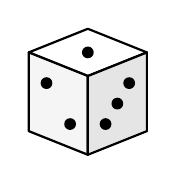
\begin{tikzpicture}[scale=0.5]
			% Style des points du dé (plus gros)
			\tikzset{ pion/.style={circle, fill=black, inner sep=1.5pt} }
			\draw[thick, fill=white, join=round]
			(0,2) -- (1.5,2.6) -- (0,3.2) -- (-1.5,2.6) -- cycle;
			\begin{scope}[cm={0.75, 0.3, -0.75, 0.3, (0, 2.6)}]
				\node[pion] at (0,0) {};
			\end{scope}
			\draw[thick, fill=gray!8, join=round]
			(0,0) -- (0,2) -- (-1.5,2.6) -- (-1.5,0.6) -- cycle;
			\begin{scope}[cm={-0.75, 0.3, 0, 1, (-0.75, 1.3)}]
				\node[pion] at (-0.4, -0.4) {};
				\node[pion] at (0.4, 0.4) {};
			\end{scope}
			\draw[thick, fill=gray!20, join=round] (0,0) -- (0,2) -- (1.5,2.6) -- (1.5,0.6) -- cycle;
			\begin{scope}[cm={0.75, 0.3, 0, 1, (0.75, 1.3)}]
				\node[pion] at (-0.4, -0.4) {};
				\node[pion] at (0, 0) {};
				\node[pion] at (0.4, 0.4) {};
			\end{scope}
		\end{tikzpicture}
	\end{wrapstuff}

	On lance le dé représenté ci-contre et on regarde le numéro inscrit sur la face du dessus.

	On ne peut pas prévoir, avant de lancer, quel numéro va sortir~: c'est une expérience aléatoire.

	\phantom{x}

	\phantom{x}
\end{ex}

\begin{defin}[Univers]
	L'ensemble de \textbf{tous} les résultats possibles d'une expérience aléatoire s'appelle l'\textbf{univers} de l'expérience.

	On le note en général $\Omega$ (la lettre grecque \og oméga \fg{}).

	Chaque résultat possible s'appelle une \textbf{issue}.
\end{defin}

\begin{ex}
	\nline
	\begin{itemize}
		\item Expérience aléatoire~: \og On lance un dé à six faces et on note le numéro obtenu \fg{}
		\item Univers~: $\Omega = \left\{ \epsdice{1};\epsdice{2};\epsdice{3};\epsdice{4};\epsdice{5};\epsdice{6} \right\}$
		\item Chacun des six résultats possibles est une \textbf{issue} de l'expérience.
	\end{itemize}
\end{ex}

\begin{defin}[Événement]
	Un \textbf{événement} est un ensemble d'issues d'une expérience aléatoire, c'est-à-dire une \textbf{partie} de l'univers $\Omega$.

	Lorsqu'un événement n'est constitué que d'une seule issue, on dit que c'est un \textbf{événement élémentaire}.
\end{defin}

\begin{ex}
	On reprend l'expérience \og lancer un dé \fg{} et $\Omega = \left\{ \epsdice{1};\epsdice{2};\epsdice{3};\epsdice{4};\epsdice{5};\epsdice{6} \right\}$.
	\begin{itemize}
		\item $A~:$ \og Obtenir un nombre pair \fg{} $\quad\Rarr\quad A = \left\{ \epsdice{2};\epsdice{4};\epsdice{6} \right\}$
		\item $B~:$ \og Obtenir un nombre supérieur ou égal à 5 \fg{} $\quad\Rarr\quad B = \left\{ \epsdice{5};\epsdice{6} \right\}$
		\item $C~:$ \og Obtenir le numéro 3 \fg{} $\quad\Rarr\quad C = \left\{ \epsdice{3} \right\}$ est un événement \textbf{élémentaire}.
	\end{itemize}
\end{ex}

\begin{rem}
	\nline
	\begin{itemize}
		\item L'événement \textbf{certain} est l'univers $\Omega$ tout entier~: il est toujours réalisé, quelle que soit l'issue obtenue.
		\item L'événement \textbf{impossible} est l'ensemble vide, noté $\varnothing$~: aucune issue ne peut le réaliser.
	\end{itemize}
\end{rem}

\begin{ex}
	Avec l'expérience aléatoire précédente~:
	\begin{itemize}
		\item \og Obtenir un nombre compris entre 1 et 6 \fg{} est l'événement \textbf{certain}.
		\item \og Obtenir le nombre 9 \fg{} est un événement \textbf{impossible}.
	\end{itemize}
\end{ex}

\begin{ex}
	\nline
	\begin{itemize}
		\item \textbf{Expérience aléatoire~:} \og On choisit un élève au hasard dans la classe et on compte son nombre de frères et s\oe{}urs \fg{} (dans une classe où personne n'en a plus de 4).
		\item \textbf{Univers~:} $\Omega = \left\{ 0 ; 1 ; 2 ; 3 ; 4 \right\}$
		\item Chaque nombre de $0$ à $4$ est une \textbf{issue} de l'expérience.
		\item \textbf{Événements~:}
		      \begin{itemize}
			      \item $A~:$ \og L'élève a au moins deux frères et s\oe{}urs \fg{} $\quad\Rarr\quad A = \left\{ 2 ; 3 ; 4 \right\}$
			      \item $B~:$ \og L'élève a un nombre pair de frères et s\oe{}urs \fg{} $\quad\Rarr\quad B = \left\{ 0 ; 2 ; 4 \right\}$
			      \item $C~:$ \og L'élève est enfant unique \fg{} $\quad\Rarr\quad C = \left\{ 0 \right\}$ est un événement \textbf{élémentaire}.
			      \item \og L'élève a moins de 5 frères et s\oe{}urs \fg{} est l'événement \textbf{certain}.
			      \item \og L'élève a 10 frères et s\oe{}urs \fg{} est un événement \textbf{impossible}.
		      \end{itemize}
	\end{itemize}
\end{ex}

\begin{ex}
	\nline
	\begin{itemize}
		\item \textbf{Expérience aléatoire~:} \og On consulte l'application météo pour relever le temps qu'il fera samedi après-midi \fg{}
		\item \textbf{Univers~:} $\Omega = \left\{ \text{Soleil} ; \text{Nuageux} ; \text{Pluie} ; \text{Neige} \right\}$
		\item Chaque type de temps est une \textbf{issue} de l'expérience.
		\item \textbf{Événements~:}
		      \begin{itemize}
			      \item $A~:$ \og Il y a des précipitations \fg{} $\quad\Rarr\quad A = \left\{ \text{Pluie} ; \text{Neige} \right\}$
			      \item $B~:$ \og Il ne pleut pas \fg{} $\quad\Rarr\quad B = \left\{ \text{Soleil} ; \text{Nuageux} ; \text{Neige} \right\}$
			      \item $C~:$ \og Il fait soleil \fg{} $\quad\Rarr\quad C = \left\{ \text{Soleil} \right\}$ est un événement \textbf{élémentaire}.
			      \item \og Le temps correspond à l'une des quatre conditions météo \fg{} est l'événement \textbf{certain}.
			      \item \og Il tombe des grenouilles \fg{} est un événement \textbf{impossible}.
		      \end{itemize}
	\end{itemize}
\end{ex}

\section{Calculer des probabilités}

\subsection{Loi de probabilité}

\begin{defin}[Loi de probabilité]
	Soit $\Omega = \left\{ e_1 ; e_2 ; \ldots ; e_n \right\}$ l'univers associé à une expérience aléatoire.

	\textbf{Définir une loi de probabilité} sur $\Omega$, c'est associer à chaque issue $e_i$ un nombre réel $p_i$, appelé \textbf{probabilité} de l'issue $e_i$ et noté $P(e_i)$, tel que~:

	\begin{itemize}
		\item Chaque probabilité est comprise entre $0$ et $1$~: $\quad 0 \le P(e_i) \le 1$
		\item La somme de toutes les probabilités vaut $1$~: $\quad P(e_1) + P(e_2) + \ldots + P(e_n) = 1$
	\end{itemize}

	On présente souvent une loi de probabilité sous forme d'un tableau.
\end{defin}

\begin{ex}
	\nline
	\begin{wrapstuff}[r]
		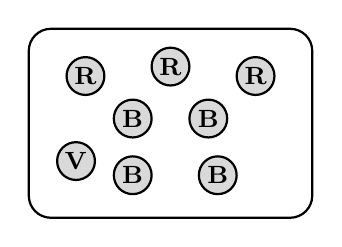
\begin{tikzpicture}[scale=0.6]
			\draw[thick, rounded corners=8pt] (-3,-2) rectangle (3,2);
			\foreach \p/\l in { (-1.8, 1.0)/R, (0.0, 1.2)/R, (1.8, 1.0)/R, (-2.0,-0.8)/V, (-0.8, 0.1)/B, (0.8, 0.1)/B, (-0.8,-1.1)/B, (1.0,-1.1)/B } { \filldraw[fill=black!15, draw=black, thick] \p circle (0.4); \node at \p {\small\textbf{\l}}; }
		\end{tikzpicture}
	\end{wrapstuff}
	Un sac opaque contient $8$ jetons indiscernables au toucher~:

	\begin{itemize}
		\item $3$ jetons rouges
		\item $1$ jeton vert
		\item $4$ jetons bleus.
	\end{itemize}

	On tire un jeton au hasard et on note sa couleur.

	La situation n'est pas équiprobable~: il y a plus de jetons bleus que de jetons verts.

	On obtient la loi de probabilité suivante~:
	\[
		\begin{array}{|c|c|c|c|} \hline
			\cellcolor{gray!30} e_i                          & \text{Rouge}           & \text{Vert}            & \text{Bleu}          \\ \hline
			\cellcolor{gray!30} \rule[-4mm]{0mm}{11mm}P(e_i) & \dfrac{3}{8} = 0{,}375 & \dfrac{1}{8} = 0{,}125 & \dfrac{4}{8} = 0{,}5 \\ \hline
		\end{array}
	\]

	On vérifie bien que~: $\quad 0{,}375 + 0{,}125 + 0{,}5 = 1$
\end{ex}

\begin{defin}[Probabilité d'un événement]
	La \textbf{probabilité} d'un événement $A$, notée $P(A)$, est la \textbf{somme} des probabilités des issues qui le composent.
\end{defin}

\begin{ex}
	\nline
	\begin{itemize}
		\item \textbf{Expérience aléatoire~:} \og On choisit une personne au hasard en France et on note son groupe sanguin (système ABO) \fg{}

		\item La loi de probabilité associée est la suivante~:

		      \begin{center}
			      \begin{tabular}{|c|c|c|c|c|} \hline
				      \cellcolor{gray!30}Groupe sanguin $e_i$ & $A$      & $O$      & $B$      & $AB$     \\ \hline
				      \cellcolor{gray!30}$P(e_i)$             & $0{,}44$ & $0{,}42$ & $0{,}10$ & $0{,}04$ \\ \hline
			      \end{tabular}
		      \end{center}
		      \ms
		\item Soit $R~:$ \og La personne possède un groupe sanguin rare (B ou AB) \fg{}, donc $R = \left\{ B ; AB \right\}$.
		      \[
			      P(R) = P(B) + P(AB) = 0{,}10 + 0{,}04 = 0{,}14
		      \]
	\end{itemize}
\end{ex}

\begin{ex}[Étude d'un jeu de dominos]
	\nline
	\begin{wrapstuff}[r]
		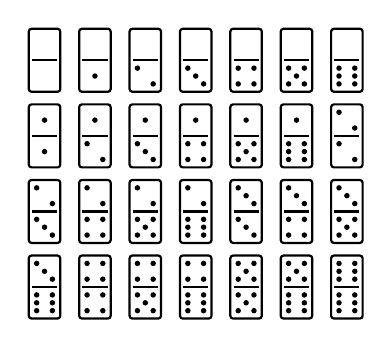
\begin{tikzpicture}[scale=0.4]
			\tikzset{ dot/.style={circle, fill=black, inner sep=0.7pt} }
			\newcommand{\drawdots}[3]{
				\ifnum#3=1
					\node[dot] at (#1,#2) {};
				\fi
				\ifnum#3=2
					\node[dot] at (#1-0.25,#2+0.25) {};
					\node[dot] at (#1+0.25,#2-0.25) {};
				\fi
				\ifnum#3=3
					\node[dot] at (#1-0.25,#2+0.25) {};
					\node[dot] at (#1,#2) {};
					\node[dot] at (#1+0.25,#2-0.25) {};
				\fi
				\ifnum#3=4
					\node[dot] at (#1-0.25,#2+0.25) {};
					\node[dot] at (#1+0.25,#2+0.25) {};
					\node[dot] at (#1-0.25,#2-0.25) {};
					\node[dot] at (#1+0.25,#2-0.25) {};
				\fi
				\ifnum#3=5
					\node[dot] at (#1-0.25,#2+0.25) {};
					\node[dot] at (#1+0.25,#2+0.25) {};
					\node[dot] at (#1,#2) {};
					\node[dot] at (#1-0.25,#2-0.25) {};
					\node[dot] at (#1+0.25,#2-0.25) {};
				\fi
				\ifnum#3=6
					\node[dot] at (#1-0.25,#2+0.25) {};
					\node[dot] at (#1+0.25,#2+0.25) {};
					\node[dot] at (#1-0.25,#2) {};
					\node[dot] at (#1+0.25,#2) {};
					\node[dot] at (#1-0.25,#2-0.25) {};
					\node[dot] at (#1+0.25,#2-0.25) {};
				\fi
			}
			\foreach \valH/\valB [count=\col from 0] in {0/0, 0/1, 0/2, 0/3, 0/4, 0/5, 0/6} {
					\pgfmathsetmacro{\x}{\col * 1.6}
					\pgfmathsetmacro{\y}{0}
					\draw[thick, rounded corners=1pt, fill=white] (\x-0.5, \y-1) rectangle (\x+0.5, \y+1);
					\draw[thick] (\x-0.4, \y) -- (\x+0.4, \y);
					\drawdots{\x}{\y+0.5}{\valH}
					\drawdots{\x}{\y-0.5}{\valB}
				}
			\foreach \valH/\valB [count=\col from 0] in {1/1, 1/2, 1/3, 1/4, 1/5, 1/6, 2/2} {
					\pgfmathsetmacro{\x}{\col * 1.6}
					\pgfmathsetmacro{\y}{-2.4}
					\draw[thick, rounded corners=1pt, fill=white] (\x-0.5, \y-1) rectangle (\x+0.5, \y+1);
					\draw[thick] (\x-0.4, \y) -- (\x+0.4, \y);
					\drawdots{\x}{\y+0.5}{\valH}
					\drawdots{\x}{\y-0.5}{\valB}
				}
			\foreach \valH/\valB [count=\col from 0] in {2/3, 2/4, 2/5, 2/6, 3/3, 3/4, 3/5} {
					\pgfmathsetmacro{\x}{\col * 1.6}
					\pgfmathsetmacro{\y}{-4.8}
					\draw[thick, rounded corners=1pt, fill=white] (\x-0.5, \y-1) rectangle (\x+0.5, \y+1);
					\draw[thick] (\x-0.4, \y) -- (\x+0.4, \y);
					\drawdots{\x}{\y+0.5}{\valH}
					\drawdots{\x}{\y-0.5}{\valB}
				}
			\foreach \valH/\valB [count=\col from 0] in {3/6, 4/4, 4/5, 4/6, 5/5, 5/6, 6/6} {
					\pgfmathsetmacro{\x}{\col * 1.6}
					\pgfmathsetmacro{\y}{-7.2}
					\draw[thick, rounded corners=1pt, fill=white] (\x-0.5, \y-1) rectangle (\x+0.5, \y+1);
					\draw[thick] (\x-0.4, \y) -- (\x+0.4, \y);
					\drawdots{\x}{\y+0.5}{\valH}
					\drawdots{\x}{\y-0.5}{\valB}
				}
		\end{tikzpicture}
	\end{wrapstuff}

	Un jeu de dominos traditionnel contient $28$ pièces distinctes marquant chacune deux nombres de points de $0$ à $6$ (du double zéro au double six).

	\begin{itemize}
		\item \textbf{Expérience aléatoire~:} \og On tire au hasard un domino dans le jeu et on calcule la somme des points inscrits sur la pièce \fg{}

		\item \textbf{Univers~:} La somme minimale possible est $0+0=0$ et la somme maximale est $6+6=12$.
		      \[ \Omega = \left\{ 0 ; 1 ; 2 ; 3 ; 4 ; 5 ; 6 ; 7 ; 8 ; 9 ; 10 ; 11 ; 12 \right\} \]
		      L'univers contient $13$ issues.

		\item \textbf{Établissement de la loi de probabilité de la somme~:}

		      Chaque domino a la même chance d'être tiré $\pa{\frac{1}{28}}$, mais certaines sommes peuvent être obtenues avec plusieurs dominos différents~:

		      \small

		      \begin{multicols}{2}
			      \begin{itemize}[itemsep=1mm]
				      \item Somme = $0$~: $\{0-0\}$  $\ \Rarr\  P(0) = \frac{1}{28}$
				      \item Somme = $1$~: $\{0-1\}$  $\ \Rarr\  P(1) = \frac{1}{28}$
				      \item Somme = $2$~: $\{0-2\,;\,1-1\}$  $\ \Rarr\  P(2) = \frac{2}{28}$
				      \item Somme = $3$~: $\{0-3\,;\,1-2\}$  $\ \Rarr\  P(3) = \frac{2}{28}$
				      \item Somme = $4$~: $\{0-4\,;\,1-3\,;\,2-2\}$  $\ \Rarr\  P(4) = \frac{3}{28}$
				      \item Somme = $5$~: $\{0-5\,;\,1-4\,;\,2-3\}$  $\ \Rarr\  P(5) = \frac{3}{28}$
				      \item Somme = $6$~: $\{0-6\,;\,1-5\,;\,2-4\,;\,3-3\}$  $\ \Rarr\  P(6) = \frac{4}{28}$
				      \item Somme = $7$~: $\{1-6\,;\,2-5\,;\,3-4\}$  $\ \Rarr\  P(7) = \frac{3}{28}$
				      \item Somme = $8$~: $\{2-6\,;\,3-5\,;\,4-4\}$  $\ \Rarr\  P(8) = \frac{3}{28}$
				      \item Somme = $9$~: $\{3-6\,;\,4-5\}$  $\ \Rarr\  P(9) = \frac{2}{28}$
				      \item Somme = $10$~: $\{4-6\,;\,5-5\}$  $\ \Rarr\  P(10) = \frac{2}{28}$
				      \item Somme = $11$~: $\{5-6\}$  $\ \Rarr\  P(11) = \frac{1}{28}$
				      \item Somme = $12$~: $\{6-6\}$  $\ \Rarr\  P(12) = \frac{1}{28}$
			      \end{itemize}
		      \end{multicols}
		      \normalsize

		      On résume la loi de probabilité dans le tableau suivant~:

		      \begin{center}
			      \rnc{\arraystretch}{1.3}
			      \begin{tabular}{|c|c|c|c|c|c|c|c|c|c|c|c|c|c|}
				      \hline
				      \cellcolor{gray!30}  $e_i$                         & $0$             & $1$             & $2$             & $3$             & $4$             & $5$             & $6$             & $7$             & $8$             & $9$             & $10$            & $11$            & $12$            \\ \hline
				      \cellcolor{gray!30} \rule[-4mm]{0mm}{10mm}$P(e_i)$ & $\dfrac{1}{28}$ & $\dfrac{1}{28}$ & $\dfrac{2}{28}$ & $\dfrac{2}{28}$ & $\dfrac{3}{28}$ & $\dfrac{3}{28}$ & $\dfrac{4}{28}$ & $\dfrac{3}{28}$ & $\dfrac{3}{28}$ & $\dfrac{2}{28}$ & $\dfrac{2}{28}$ & $\dfrac{1}{28}$ & $\dfrac{1}{28}$ \\ \hline
			      \end{tabular}
		      \end{center}

		      \ms

		\item \textbf{Calcul de la probabilité d'un événement~:}

		      Soit $S~:$ \og Obtenir un domino dont la somme des points est strictement supérieure à $7$ \fg{}.

		      Les issues composant l'événement $S$ sont $S = \left\{ 8 ; 9 ; 10 ; 11 ; 12 \right\}$.

		      Par définition, $P(S)$ est la \textbf{somme des probabilités des issues} qui le composent~:
		      \[
			      \def\arraystretch{1.5}
			      \begin{array}{rccccccccccl}
				      P(S) & = & P(8)          & + & P(9)          & + & P(10)         & + & P(11)         & + & P(12)         &                 \\
				           & = & \dfrac{3}{28} & + & \dfrac{2}{28} & + & \dfrac{2}{28} & + & \dfrac{1}{28} & + & \dfrac{1}{28} & = \dfrac{9}{28}
			      \end{array}
		      \]
		      La probabilité de tirer un domino dont la somme des points est supérieure à $7$ est donc égale à $\dfrac{9}{28}$.
	\end{itemize}
\end{ex}
\subsection{Événement contraire}

\begin{defin}[Événement contraire]
	Soit $A$ un événement d'un univers $\Omega$.

	L'\textbf{événement contraire} de $A$, noté $\bar{A}$ (et lu \og $A$ barre \fg{}), est l'événement constitué de toutes les issues de $\Omega$ qui \textbf{n'appartiennent pas} à $A$.
\end{defin}

\begin{prop}[Probabilité de l'événement contraire]
	Pour tout événement $A$, la somme des probabilités de $A$ et de son contraire est égale à $1$~:
	\[ P\pa{A} + P\pa{\bar{A}} = 1 \quad\Rarr\quad P\pa{\bar{A}} = 1 - P(A) \]
\end{prop}

\begin{ex}[Calcul à l'aide de l'événement contraire]
	On reprend le jeu de $28$ dominos de l'exemple précédent. On tire un domino au hasard.

	Soit $E$ l'événement~: \og Obtenir un domino dont la somme des points est au moins égale à $2$ \fg{}.

	\begin{itemize}
		\item Calculer directement $P(E)$ nécessiterait d'additionner les probabilités des issues $2, 3, 4, 5, 6, 7, 8, 9, 10, 11$ et $12$ ($11$ calculs).

		\item L'événement contraire de $E$ est $\bar{E}~:$ \og Obtenir une somme strictement inférieure à $2$ \fg{}.

		      Les seules issues réalisant $\bar{E}$ sont $0$ et $1$, soit $\bar{E} = \left\{ 0 ; 1 \right\}$.

		\item On calcule facilement la probabilité de $\bar{E}$~:
		      \[ P\pa{\bar{E}} = P(0) + P(1) = \dfrac{1}{28} + \dfrac{1}{28} = \dfrac{2}{28} \]

		\item On en déduit alors la probabilité de $E$~:
		      \[ P(E) = 1 - P\pa{\bar{E}} = 1 - \dfrac{2}{28} = \dfrac{26}{28} = \dfrac{13}{14} \]
	\end{itemize}
\end{ex}

\subsection{Situations d'équiprobabilité}

\begin{defin}[Équiprobabilité]
	On dit qu'il y a \textbf{équiprobabilité} lorsque toutes les issues de l'univers ont la \textbf{même} probabilité de se réaliser.

	On dit aussi que la loi de probabilité est \textbf{équirépartie}.
\end{defin}

\begin{prop}
	Dans une situation d'équiprobabilité sur un univers $\Omega$ constitué de $n$ issues, la probabilité d'un événement $A$ est~:
	\[
		P(A) = \dfrac{\text{nombre d'issues favorables à } A}{\text{nombre d'issues total}} = \dfrac{\text{Card}(A)}{\text{Card}(\Omega)}
	\]

	\ldots où $\text{Card}(A)$ désigne le \textbf{cardinal} de l'ensemble $A$, c'est-à-dire son nombre d'éléments (d'issues).
\end{prop}

\begin{ex}
	On tire au hasard une carte dans un jeu de $32$ cartes bien mélangé.
	\begin{itemize}
		\item L'univers est $\Omega = \left\{ \text{7 de C\oe{}ur} ; \text{8 de C\oe{}ur} ; \ldots ; \text{As de Pique} \right\}$ et contient $32$ issues.
		\item Toutes les cartes ont la même chance d'être tirées~: il y a \textbf{équiprobabilité}.
		\item La probabilité de tirer une carte précise (par exemple l'As de C\oe{}ur) est $P(\text{\og As de C\oe{}ur \fg{}}) = \dfrac{1}{32}$.
	\end{itemize}
\end{ex}

\begin{ex}
	On lance un dé \textbf{non truqué} à six faces. Toutes les faces ont la même chance de sortir~: la situation est équiprobable, et $P\pa{\epsdice{1}} = P\pa{\epsdice{2}} = \ldots = P\pa{\epsdice{6}} = \dfrac{1}{6}$.

	Soit $A~:$ \og Obtenir un multiple de 3 \fg{}, donc $A = \left\{ \epsdice{3};\epsdice{6} \right\}$.
	\[
		P(A) = \dfrac{\text{Card}(A)}{\text{Card}(\Omega)} = \dfrac{2}{6} = \dfrac{1}{3}
	\]
\end{ex}

\section{Intersection et union d'événements}

\begin{defin}[Intersection d'événements]
	Soient $A$ et $B$ deux événements d'un même univers $\Omega$.

	L'\textbf{intersection} des événements $A$ et $B$, notée $A \cap B$ (et lue \og $A$ inter $B$ \fg{}), est l'événement constitué des issues qui appartiennent \textbf{à la fois} à $A$ \textbf{et} à $B$.
\end{defin}

\begin{defin}[Union d'événements]
	Soient $A$ et $B$ deux événements d'un même univers $\Omega$.

	L'\textbf{union} des événements $A$ et $B$, notée $A \cup B$ (et lue \og $A$ union $B$ \fg{}), est l'événement constitué des issues qui appartiennent à $A$, à $B$, \textbf{ou aux deux}.
\end{defin}

\begin{rem}
	En mathématiques, le \og ou \fg{} est inclusif~: réaliser $A \cup B$ signifie réaliser $A$, réaliser $B$, ou réaliser les deux en même temps.
\end{rem}

\begin{ex}[Intersection et tableau à double entrée]
	Dans une classe de Seconde de $30$ élèves, on étudie le type de téléphone portable possédé par chacun.

	On choisit un élève au hasard dans la classe.

	La répartition des élèves est résumée dans le tableau à double entrée ci-dessous~:

	\begin{center}
		\rnc{\arraystretch}{1.3}
		\begin{tabular}{|c|c|c|c|}
			\hline
			\cellcolor{gray!30}   & \cellcolor{gray!30}Téléphone Pomme $\pa{P}$ & \cellcolor{gray!30}Autre marque $\pa{\bar{P}}$ & \cellcolor{gray!30}\textbf{Total} \\ \hline
			Fille $\pa{F}$        & $12$                                        & $6$                                            & \textbf{18}                       \\ \hline
			Garçon $\pa{\bar{F}}$ & $4$                                         & $8$                                            & \textbf{12}                       \\ \hline
			\textbf{Total}        & \textbf{16}                                 & \textbf{14}                                    & \textbf{30}                       \\ \hline
		\end{tabular}
	\end{center}

	On considère les événements suivants~:
	\begin{itemize}
		\item $F~:$ \og L'élève choisi est une fille \fg{}
		\item $P~:$ \og L'élève choisi a un téléphone Pomme \fg{}
	\end{itemize}

	Chaque élève a la même chance d'être choisi (équiprobabilité), donc~:
	\begin{itemize}
		\item Probabilité que l'élève soit une fille~:
		      \[ P(F) = \dfrac{\text{Card}(F)}{\text{Card}(\Omega)} = \dfrac{18}{30} = 0{,}6 \]
		\item Probabilité que l'élève ait un téléphone Pomme~:
		      \[ P(P) = \dfrac{\text{Card}(P)}{\text{Card}(\Omega)} = \dfrac{16}{30} = \dfrac{8}{15} \approx 0{,}533 \]
		\item L'événement $F \cap P$ est \og L'élève est une fille \textbf{et} a un téléphone Pomme \fg{}.

		      D'après le tableau, $12$ élèves correspondent à ce profil~:
		      \[ P(F \cap P) = \dfrac{\text{Card}(F \cap P)}{\text{Card}(\Omega)} = \dfrac{12}{30} = 0{,}4 \]
	\end{itemize}
\end{ex}

\begin{prop}[Calcul de la probabilité de l'union]
	Soient $A$ et $B$ deux événements d'un même univers $\Omega$.

	La probabilité de l'événement $A \cup B$ est donnée par la formule~:
	\[ P(A \cup B) = P(A) + P(B) - P(A \cap B) \]
\end{prop}

\begin{rem}
	On soustrait $P(A \cap B)$ pour ne pas compter deux fois les issues qui sont communes à $A$ et à $B$.
\end{rem}

\begin{ex}[Exemple avec la formule de l'union]
	Lors d'une compétition de jeux vidéo (E-sport), $100$ joueurs s'affrontent.
	\begin{itemize}
		\item $60$ joueurs jouent sur Console~;
		\item $50$ joueurs jouent sur PC~;
		\item $20$ joueurs jouent à la fois sur Console et sur PC.
	\end{itemize}

	On choisit un joueur au hasard. On note :
	\begin{itemize}
		\item $C$ l'événement \og Le joueur joue sur Console \fg{}
		\item $K$ l'événement \og Le joueur joue sur PC \fg{}.
	\end{itemize}

	On a donc $P(C) = \frac{60}{100} = 0{,}6$, $\quad P(K) = \frac{50}{100} = 0{,}5 \quad$ et $\quad P(C \cap K) = \frac{20}{100} = 0{,}2$.

	\ms

	On cherche la probabilité $P(C \cup K)$ que le joueur joue sur au moins un de ces deux supports~:
	\[ P(C \cup K) = P(C) + P(B) - P(C \cap K) = 0{,}6 + 0{,}5 - 0{,}2 = 0{,}9 \]

	Il y a donc $90\,\%$ de chances que le joueur sélectionné joue sur PC ou sur Console.
\end{ex}

\begin{ex}
	Un festival de musique propose un stand de prévention contre le bruit.

	Sur $200$ festivaliers interrogés à la sortie~:

	\begin{itemize}
		\item $140$ portent des bouchons d'oreilles $\pa{B}$~;
		\item $80$ font des pauses régulières hors du son $\pa{P}$~;
		\item $50$ font les deux $\pa{B \cap P}$.
	\end{itemize}

	On choisit un festivalier au hasard.

	La probabilité qu'il adopte \textbf{au moins un} des deux réflexes de prévention est $P(B \cup P)$~:
	\[ P(B \cup P) = P(B) + P(P) - P(B \cap P) = \dfrac{140}{200} + \dfrac{80}{200} - \dfrac{50}{200} = \dfrac{170}{200} = 0{,}85 \]
\end{ex}

\subsection{Représentation par un diagramme de Venn}

\begin{defin}[Diagramme de Venn]
	Un \textbf{diagramme de Venn} est une représentation graphique dans laquelle l'univers $\Omega$ est représenté par un ensemble fermé (souvent un rectangle ou une grande ellipse), et les événements par des ensembles géométriques (souvent des cercles) qui se chevauchent.
\end{defin}

\begin{ex}[Diagramme de Venn et langues vivantes]
	Dans une classe de $35$ élèves de Seconde~:
	\begin{itemize}
		\item $20$ élèves étudient l'Espagnol ($E$)~;
		\item $12$ élèves étudient l'Allemand ($A$)~;
		\item $5$ élèves étudient à la fois l'Espagnol et l'Allemand ($E \cap A$)~;
	\end{itemize}

	\begin{center}
		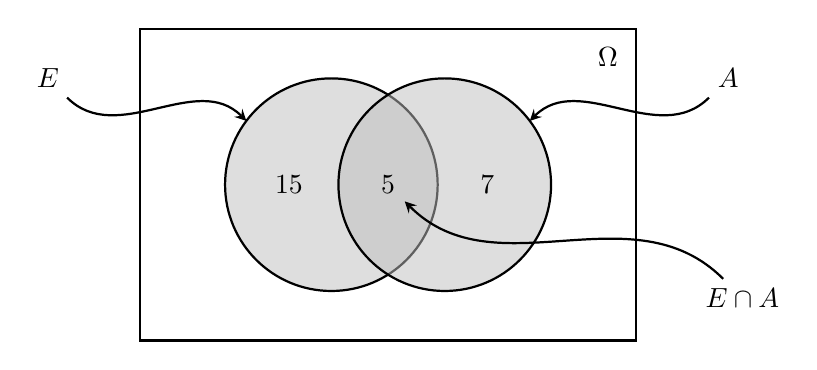
\begin{tikzpicture}[scale=0.9]
			\draw[thick, fill=white] (-3.5,-2.2) rectangle (3.5,2.2);
			\node at (3.1,1.8) {$\Omega$};
			\draw[thick, fill=gray!50, fill opacity=0.5] (-0.8,0) circle (1.5);
			\draw[thick, fill=gray!50, fill opacity=0.5] (0.8,0) circle (1.5);
			\node at (-1.4,0) {$15$};
			\node (inter) at (0,0) {$5$};
			\node at (1.4,0) {$7$};
			\node (nodeE) at (-4.8,1.5) {\textbf{$E$}};
			\draw[->, >=stealth, thick] (nodeE) to[out=-45, in=135] (-2,0.9);
			\node (nodeA) at (4.8,1.5) {\textbf{$A$}};
			\draw[->, >=stealth, thick] (nodeA) to[out=-135, in=45] (2,0.9);
			\node (nodeInter) at (5,-1.6) {\textbf{$E \cap A$}};
			\draw[->, >=stealth, thick] (nodeInter) to[out=135, in=-45] (inter);
		\end{tikzpicture}
	\end{center}

	On choisit un élève au hasard.

	Grâce au diagramme, on lit directement la répartition des effectifs disjoints~:
	\begin{itemize}
		\item Probabilité que l'élève étudie l'Espagnol \textbf{et} l'Allemand~:
		      \[ P(E \cap A) = \dfrac{\text{Card}(E \cap A)}{\text{Card}(\Omega)} = \dfrac{5}{35} = \dfrac{1}{7} \]
		\item Probabilité que l'élève étudie \textbf{uniquement} l'Espagnol~:
		      \[ P(E \setminus A) = \dfrac{20 - 5}{35} = \dfrac{15}{35} = \dfrac{3}{7} \]
		\item Probabilité que l'élève étudie \textbf{au moins une} des deux langues~:
		      \[ P(E \cup A) = \dfrac{15 + 5 + 7}{35} = \dfrac{27}{35} \]
		\item Probabilité que l'élève n'étudie \textbf{aucune} de ces deux langues~:
		      \[ P\pa{\bar{E \cup A}} = 1 - P(E \cup A) = 1 - \dfrac{27}{35} = \dfrac{8}{35} \]
	\end{itemize}
\end{ex}
